This paper addresses the problem of Passive Global Localisation of a 2D LIDAR
sensor, i.e. the estimation of its location and orientation within a given map,
under complete locational and orientational uncertainty, without prescribing
motion commands (to the mobile robot that the sensor is assumed mounted to) for
further knowledge acquisition. The problem is formalised in Problem
\ref{prob:the_problem}:

%%%%%%%%%%%%%%%%%%%%%%%%%%%%%%%%%%%%%%%%%%%%%%%%%%%%%%%%%%%%%%%%%%%%%%%%%%%%%%%%
\begin{customprb}{P}
  \label{prob:the_problem}
  Let the unknown pose of an immobile 2D range sensor whose angular range is
  $\lambda$ be $\bm{p}(\bm{l},\theta)$, $\bm{l} = (x,y)$, with respect to the
  reference frame of map $\bm{M}$. Let the range sensor measure range scan
  $\mathcal{S}_R$. The objective is the estimation of $\bm{p}$ given $\bm{M}$,
  $\lambda$, and $\mathcal{S}_R$.
\end{customprb}
%%%%%%%%%%%%%%%%%%%%%%%%%%%%%%%%%%%%%%%%%%%%%%%%%%%%%%%%%%%%%%%%%%%%%%%%%%%%%%%%

\begin{figure}\vspace{0.4em}
  \subfloat{% GNUPLOT: LaTeX picture with Postscript
\begingroup
  \makeatletter
  \providecommand\color[2][]{%
    \GenericError{(gnuplot) \space\space\space\@spaces}{%
      Package color not loaded in conjunction with
      terminal option `colourtext'%
    }{See the gnuplot documentation for explanation.%
    }{Either use 'blacktext' in gnuplot or load the package
      color.sty in LaTeX.}%
    \renewcommand\color[2][]{}%
  }%
  \providecommand\includegraphics[2][]{%
    \GenericError{(gnuplot) \space\space\space\@spaces}{%
      Package graphicx or graphics not loaded%
    }{See the gnuplot documentation for explanation.%
    }{The gnuplot epslatex terminal needs graphicx.sty or graphics.sty.}%
    \renewcommand\includegraphics[2][]{}%
  }%
  \providecommand\rotatebox[2]{#2}%
  \@ifundefined{ifGPcolor}{%
    \newif\ifGPcolor
    \GPcolorfalse
  }{}%
  \@ifundefined{ifGPblacktext}{%
    \newif\ifGPblacktext
    \GPblacktexttrue
  }{}%
  % define a \g@addto@macro without @ in the name:
  \let\gplgaddtomacro\g@addto@macro
  % define empty templates for all commands taking text:
  \gdef\gplfronttext{}%
  \gdef\gplfronttext{}%
  \makeatother
  \ifGPblacktext
    % no textcolor at all
    \def\colorrgb#1{}%
    \def\colorgray#1{}%
  \else
    % gray or color?
    \ifGPcolor
      \def\colorrgb#1{\color[rgb]{#1}}%
      \def\colorgray#1{\color[gray]{#1}}%
      \expandafter\def\csname LTw\endcsname{\color{white}}%
      \expandafter\def\csname LTb\endcsname{\color{black}}%
      \expandafter\def\csname LTa\endcsname{\color{black}}%
      \expandafter\def\csname LT0\endcsname{\color[rgb]{1,0,0}}%
      \expandafter\def\csname LT1\endcsname{\color[rgb]{0,1,0}}%
      \expandafter\def\csname LT2\endcsname{\color[rgb]{0,0,1}}%
      \expandafter\def\csname LT3\endcsname{\color[rgb]{1,0,1}}%
      \expandafter\def\csname LT4\endcsname{\color[rgb]{0,1,1}}%
      \expandafter\def\csname LT5\endcsname{\color[rgb]{1,1,0}}%
      \expandafter\def\csname LT6\endcsname{\color[rgb]{0,0,0}}%
      \expandafter\def\csname LT7\endcsname{\color[rgb]{1,0.3,0}}%
      \expandafter\def\csname LT8\endcsname{\color[rgb]{0.5,0.5,0.5}}%
    \else
      % gray
      \def\colorrgb#1{\color{black}}%
      \def\colorgray#1{\color[gray]{#1}}%
      \expandafter\def\csname LTw\endcsname{\color{white}}%
      \expandafter\def\csname LTb\endcsname{\color{black}}%
      \expandafter\def\csname LTa\endcsname{\color{black}}%
      \expandafter\def\csname LT0\endcsname{\color{black}}%
      \expandafter\def\csname LT1\endcsname{\color{black}}%
      \expandafter\def\csname LT2\endcsname{\color{black}}%
      \expandafter\def\csname LT3\endcsname{\color{black}}%
      \expandafter\def\csname LT4\endcsname{\color{black}}%
      \expandafter\def\csname LT5\endcsname{\color{black}}%
      \expandafter\def\csname LT6\endcsname{\color{black}}%
      \expandafter\def\csname LT7\endcsname{\color{black}}%
      \expandafter\def\csname LT8\endcsname{\color{black}}%
    \fi
  \fi
    \setlength{\unitlength}{0.0500bp}%
    \ifx\gptboxheight\undefined%
      \newlength{\gptboxheight}%
      \newlength{\gptboxwidth}%
      \newsavebox{\gptboxtext}%
    \fi%
    \setlength{\fboxrule}{0.5pt}%
    \setlength{\fboxsep}{1pt}%
\begin{picture}(5000.00,3000.00)%
    \gplgaddtomacro\gplfronttext{%
    }%
    \gplgaddtomacro\gplfronttext{%
    }%
    \gplgaddtomacro\gplfronttext{%
    }%
    \gplgaddtomacro\gplfronttext{%
      \colorrgb{0.15,0.15,0.15}%
      \put(475,1279){\makebox(0,0)[r]{\strut{}$0$}}%
      \colorrgb{0.15,0.15,0.15}%
      %\put(791,1256){\makebox(0,0)[r]{\strut{}$5$}}%
      \colorrgb{0.15,0.15,0.15}%
      \put(1107,1233){\makebox(0,0)[r]{\strut{}$10$}}%
      \colorrgb{0.15,0.15,0.15}%
      %\put(1424,1209){\makebox(0,0)[r]{\strut{}$15$}}%
      \colorrgb{0.15,0.15,0.15}%
      \put(1740,1186){\makebox(0,0)[r]{\strut{}$20$}}%
      \colorrgb{0.15,0.15,0.15}%
      %\put(2056,1163){\makebox(0,0)[r]{\strut{}$25$}}%
      \colorrgb{0.15,0.15,0.15}%
      \put(2373,1140){\makebox(0,0)[r]{\strut{}$30$}}%
      \colorrgb{0.15,0.15,0.15}%
      %\put(2688,1117){\makebox(0,0)[r]{\strut{}$35$}}%
      \colorrgb{0.15,0.15,0.15}%
      \put(3004,1094){\makebox(0,0)[r]{\strut{}$40$}}%
      \colorrgb{0.15,0.15,0.15}%
      \put(3528,1236){\makebox(0,0)[l]{\strut{}$0$}}%
      \colorrgb{0.15,0.15,0.15}%
      %\put(3764,1366){\makebox(0,0)[l]{\strut{}$5$}}%
      \colorrgb{0.15,0.15,0.15}%
      \put(4000,1496){\makebox(0,0)[l]{\strut{}$10$}}%
      \colorrgb{0.15,0.15,0.15}%
      %\put(4236,1626){\makebox(0,0)[l]{\strut{}$15$}}%
      \colorrgb{0.15,0.15,0.15}%
      \put(4471,1756){\makebox(0,0)[l]{\strut{}$20$}}%
      \colorrgb{0.15,0.15,0.15}%
      \put(473,2125){\makebox(0,0)[r]{\strut{}$0.0$}}%
      \colorrgb{0.15,0.15,0.15}%
      \put(473,1817){\makebox(0,0)[r]{\strut{}$2.0$}}%
      \colorrgb{0.15,0.15,0.15}%
      \put(473,1509){\makebox(0,0)[r]{\strut{}$4.0$}}%
    }%
    \put(0,0){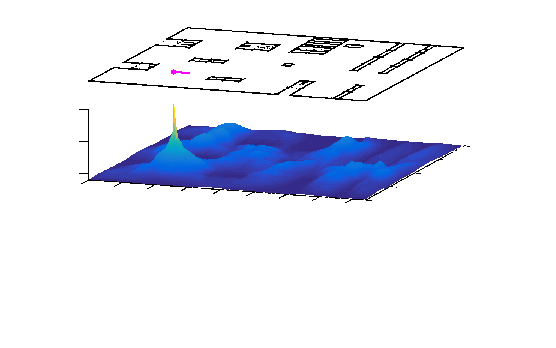
\includegraphics{./figures/face_top}}%
    \gplfronttext
  \end{picture}%
\endgroup
    \label{fig:a}} \vspace{-1.7cm}\\
  \subfloat{\hspace{-0.3cm}% GNUPLOT: LaTeX picture with Postscript
\begingroup
  \makeatletter
  \providecommand\color[2][]{%
    \GenericError{(gnuplot) \space\space\space\@spaces}{%
      Package color not loaded in conjunction with
      terminal option `colourtext'%
    }{See the gnuplot documentation for explanation.%
    }{Either use 'blacktext' in gnuplot or load the package
      color.sty in LaTeX.}%
    \renewcommand\color[2][]{}%
  }%
  \providecommand\includegraphics[2][]{%
    \GenericError{(gnuplot) \space\space\space\@spaces}{%
      Package graphicx or graphics not loaded%
    }{See the gnuplot documentation for explanation.%
    }{The gnuplot epslatex terminal needs graphicx.sty or graphics.sty.}%
    \renewcommand\includegraphics[2][]{}%
  }%
  \providecommand\rotatebox[2]{#2}%
  \@ifundefined{ifGPcolor}{%
    \newif\ifGPcolor
    \GPcolorfalse
  }{}%
  \@ifundefined{ifGPblacktext}{%
    \newif\ifGPblacktext
    \GPblacktexttrue
  }{}%
  % define a \g@addto@macro without @ in the name:
  \let\gplgaddtomacro\g@addto@macro
  % define empty templates for all commands taking text:
  \gdef\gplfronttext{}%
  \gdef\gplfronttext{}%
  \makeatother
  \ifGPblacktext
    % no textcolor at all
    \def\colorrgb#1{}%
    \def\colorgray#1{}%
  \else
    % gray or color?
    \ifGPcolor
      \def\colorrgb#1{\color[rgb]{#1}}%
      \def\colorgray#1{\color[gray]{#1}}%
      \expandafter\def\csname LTw\endcsname{\color{white}}%
      \expandafter\def\csname LTb\endcsname{\color{black}}%
      \expandafter\def\csname LTa\endcsname{\color{black}}%
      \expandafter\def\csname LT0\endcsname{\color[rgb]{1,0,0}}%
      \expandafter\def\csname LT1\endcsname{\color[rgb]{0,1,0}}%
      \expandafter\def\csname LT2\endcsname{\color[rgb]{0,0,1}}%
      \expandafter\def\csname LT3\endcsname{\color[rgb]{1,0,1}}%
      \expandafter\def\csname LT4\endcsname{\color[rgb]{0,1,1}}%
      \expandafter\def\csname LT5\endcsname{\color[rgb]{1,1,0}}%
      \expandafter\def\csname LT6\endcsname{\color[rgb]{0,0,0}}%
      \expandafter\def\csname LT7\endcsname{\color[rgb]{1,0.3,0}}%
      \expandafter\def\csname LT8\endcsname{\color[rgb]{0.5,0.5,0.5}}%
    \else
      % gray
      \def\colorrgb#1{\color{black}}%
      \def\colorgray#1{\color[gray]{#1}}%
      \expandafter\def\csname LTw\endcsname{\color{white}}%
      \expandafter\def\csname LTb\endcsname{\color{black}}%
      \expandafter\def\csname LTa\endcsname{\color{black}}%
      \expandafter\def\csname LT0\endcsname{\color{black}}%
      \expandafter\def\csname LT1\endcsname{\color{black}}%
      \expandafter\def\csname LT2\endcsname{\color{black}}%
      \expandafter\def\csname LT3\endcsname{\color{black}}%
      \expandafter\def\csname LT4\endcsname{\color{black}}%
      \expandafter\def\csname LT5\endcsname{\color{black}}%
      \expandafter\def\csname LT6\endcsname{\color{black}}%
      \expandafter\def\csname LT7\endcsname{\color{black}}%
      \expandafter\def\csname LT8\endcsname{\color{black}}%
    \fi
  \fi
    \setlength{\unitlength}{0.0500bp}%
    \ifx\gptboxheight\undefined%
      \newlength{\gptboxheight}%
      \newlength{\gptboxwidth}%
      \newsavebox{\gptboxtext}%
    \fi%
    \setlength{\fboxrule}{0.5pt}%
    \setlength{\fboxsep}{1pt}%
\begin{picture}(5000.00,3000.00)%
    \gplgaddtomacro\gplfronttext{%
    }%
    \gplgaddtomacro\gplfronttext{%
      \colorrgb{0.15,0.15,0.15}%
      \put(336,1498){\makebox(0,0)[r]{\strut{}}}%
      \colorrgb{0.15,0.15,0.15}%
      \put(336,1905){\makebox(0,0)[r]{\strut{}}}%
      \colorrgb{0.15,0.15,0.15}%
      \put(336,2312){\makebox(0,0)[r]{\strut{}}}%
      \colorrgb{0.15,0.15,0.15}%
      \put(300,1905){\rotatebox{90}{\makebox(0,0){\strut{}$\Delta\hat{\theta} \in [-\pi,\pi)$ rad}}}%
      %\put(400,933){\makebox(0,0){\strut{}\small $0.0$}}%
      \colorrgb{0.15,0.15,0.15}%
      \put(871,933){\makebox(0,0){\strut{}\small $0.5$}}%
      \colorrgb{0.15,0.15,0.15}%
      \put(1342,933){\makebox(0,0){\strut{}\small $1.0$}}%
      \colorrgb{0.15,0.15,0.15}%
      \put(1813,933){\makebox(0,0){\strut{}\small $1.5$}}%
      \colorrgb{0.15,0.15,0.15}%
      \put(2285,933){\makebox(0,0){\strut{}\small $2.0$}}%
      \colorrgb{0.15,0.15,0.15}%
      \put(1487,663){\makebox(0,0){\strut{}$\|\Delta \hat{\bm{l}}\|_2$ [m]}}%
    }%
    \gplgaddtomacro\gplfronttext{%
    }%
    \gplgaddtomacro\gplfronttext{%
      \colorrgb{0.15,0.15,0.15}%
      \put(5113,1110){\makebox(0,0)[l]{\strut{}}}%
      \colorrgb{0.15,0.15,0.15}%
      \put(5113,1110){\makebox(0,0)[l]{\strut{}}}%
      \colorrgb{0.15,0.15,0.15}%
      \put(5113,1110){\makebox(0,0)[l]{\strut{}}}%
      %\put(2875,933){\makebox(0,0){\strut{}\small $0.0$}}%
      \colorrgb{0.15,0.15,0.15}%
      \put(3346,933){\makebox(0,0){\strut{}\small $0.5$}}%
      \colorrgb{0.15,0.15,0.15}%
      \put(3817,933){\makebox(0,0){\strut{}\small $1.0$}}%
      \colorrgb{0.15,0.15,0.15}%
      \put(4288,933){\makebox(0,0){\strut{}\small $1.5$}}%
      \colorrgb{0.15,0.15,0.15}%
      \put(4760,933){\makebox(0,0){\strut{}\small $2.0$}}%
      \colorrgb{0.15,0.15,0.15}%
      \put(2762,1905){\rotatebox{90}{\makebox(0,0){\strut{}\small CAER [m]}}}
      \put(3987,663){\makebox(0,0){\strut{}$\|\Delta \hat{\bm{l}}\|_2$ [m]}}%
    }%
    \gplgaddtomacro\gplfronttext{%
    }%
    \gplgaddtomacro\gplfronttext{%
    }%
    \gplgaddtomacro\gplfronttext{%
    }%
    \gplgaddtomacro\gplfronttext{%
      \put(500,80){\makebox(0,0){\strut{}$\footnotesize 0$}}%
      \colorrgb{0.15,0.15,0.15}%
%      \put(1390,80){\makebox(0,0){\strut{}$\footnotesize 60$}}%
      %\colorrgb{0.15,0.15,0.15}%
      %\put(2280,80){\makebox(0,0){\strut{}$\footnotesize 270$}}%
      %\colorrgb{0.15,0.15,0.15}%
      %\put(3169,80){\makebox(0,0){\strut{}$\footnotesize 540$}}%
      %\colorrgb{0.15,0.15,0.15}%
      %\put(4059,80){\makebox(0,0){\strut{}$\footnotesize 810$}}%
      \colorrgb{0.15,0.15,0.15}%
      \put(4849,80){\makebox(0,0){\strut{}$\footnotesize 1080$}}%
    }%
    \put(0,0){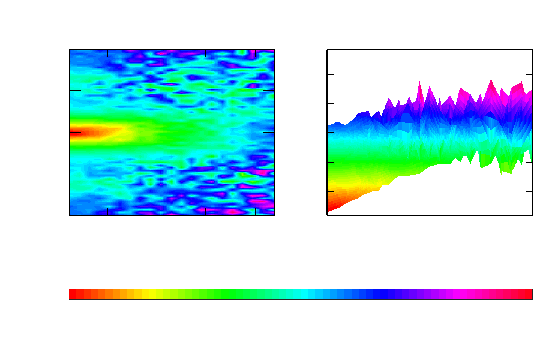
\includegraphics{./figures/face_bottom}}%
    \gplfronttext
  \end{picture}%
\endgroup
 \label{fig:b}}
  \caption{\small Top: a map of an
           environment, the pose of a panoramic 2D LIDAR sensor (magenta), and
           the corresponding CAER rank field below them. Bottom: distribution
           of CAER values by location $\Delta \hat{\bm{l}}$ and orientation
           error $\Delta \hat{\theta}$ of all sensor pose hypotheses
           corresponding to the rank field above, for estimate position errors
           up to $2.0$ m. In this example $10^6$ hypotheses are dispersed
           randomly in the free space of a map with area $735$ m$^2$, for $100$
           independent trials; CBGL's maximum location error and maximum
           execution time are, respectively, $0.062$ m and $8.8$ sec }
  \vspace{-0.75cm}
  \label{fig:face}
\end{figure}

The rest of the paper is structured as follows: Section
\ref{section:definitions} provides necessary definitions and the notation
employed. Section \ref{section:sota} gives a brief review of the
literature of solutions to problem \ref{prob:the_problem}, and the relation of
the proposed method to them.  The latter's methodology is presented in section
\ref{section:the_proposed_method}, its evaluation in section
\ref{section:results}, and its limitations in section
\ref{section:characterisation}. Section \ref{section:finale} concludes this
study.
